\begin{figure}
    \centering
    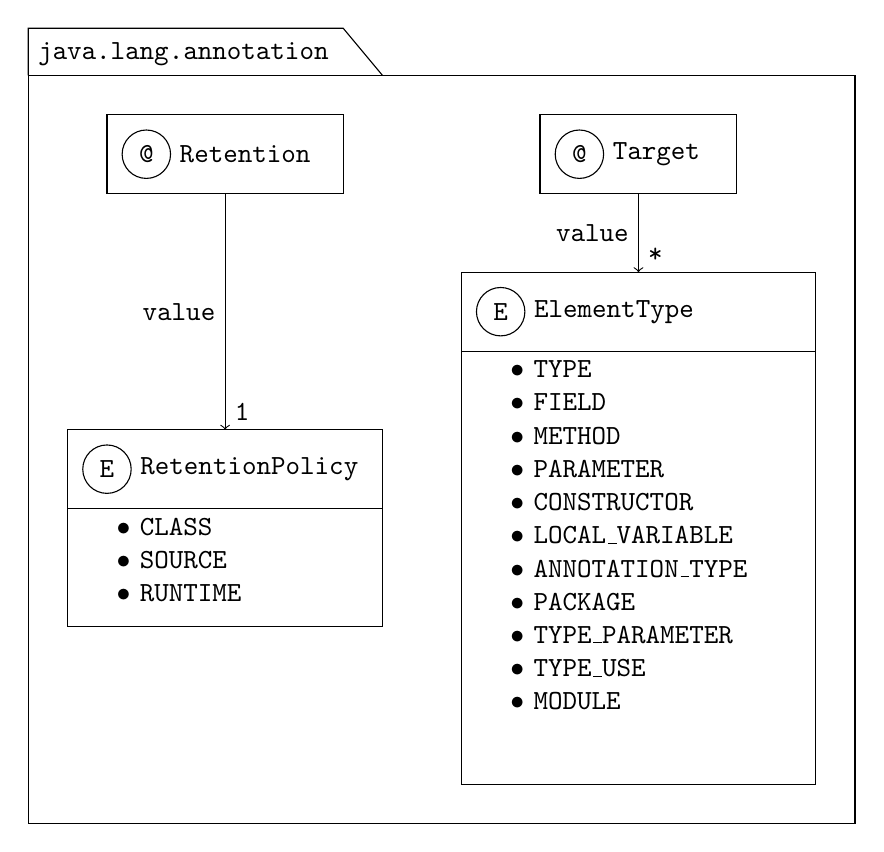
\begin{tikzpicture}
        % \draw[draw=black!20] (0, -0.5) grid (10, 10);
        \draw (0, 9) -- (0, 9.6) -- (4, 9.6) -- (4.5, 9);
        \draw (0, -0.5) rectangle (10.5, 9);
        \node[draw=none, above right] (package-name) at (0, 9) {\texttt{java.lang.annotation}};

        \node[circle, draw] (annotation-id) at (1.5, 8) {\texttt{@}};
        \node[draw=none, right=3mm] (annotation-label) at (1.5, 8) {\texttt{Retention}};
        \draw (1, 7.5) rectangle (4, 8.5);

        \node[circle, draw] (annotation-id) at (7, 8) {\texttt{@}};
        \node[draw=none, right=3mm] (annotation-label) at (7, 8) {\texttt{Target}};
        \draw (6.5, 7.5) rectangle (9, 8.5);

        \node[circle, draw] (annotation-id) at (1, 4) {\texttt{E}};
        \node[draw=none, right=3mm] (annotation-label) at (1, 4) {\texttt{RetentionPolicy}};
        \draw (0.5, 3.5) rectangle (4.5, 4.5);
        \draw (0.5, 3.5) -- (0.5, 2) -- (4.5, 2) -- (4.5, 3.5);
        \node[align=left, below right] (members) at (1, 3.5) {
            $\bullet$~\texttt{CLASS}\\
            $\bullet$~\texttt{SOURCE}\\
            $\bullet$~\texttt{RUNTIME}\\
        };

        \node[circle, draw] (annotation-id) at (6, 6) {\texttt{E}};
        \node[draw=none, right=3mm] (annotation-label) at (6, 6) {\texttt{ElementType}};
        \draw (5.5, 5.5) rectangle (10, 6.5);
        \draw (5.5, 5.5) -- (5.5, 0) -- (10, 0) -- (10, 5.5);
        \node[align=left, below right] (members) at (6, 5.5) {
            $\bullet$~\texttt{TYPE}\\
            $\bullet$~\texttt{FIELD}\\
            $\bullet$~\texttt{METHOD}\\
            $\bullet$~\texttt{PARAMETER}\\
            $\bullet$~\texttt{CONSTRUCTOR}\\
            $\bullet$~\texttt{LOCAL\_VARIABLE}\\
            $\bullet$~\texttt{ANNOTATION\_TYPE}\\
            $\bullet$~\texttt{PACKAGE}\\
            $\bullet$~\texttt{TYPE\_PARAMETER}\\
            $\bullet$~\texttt{TYPE\_USE}\\
            $\bullet$~\texttt{MODULE}\\
        };

        \draw[->] (2.5, 7.5) -- node[left] {\texttt{value}} (2.5, 4.5) node[above right] {\texttt{1}};
        \draw[->] (7.75, 7.5) -- node[left] {\texttt{value}} (7.75, 6.5) node[above right] {\texttt{*}};

    \end{tikzpicture}
    \caption{\texttt{java.lang.annotation} class diagram.}
    \label{fig:java-annotation-class-dia}
\end{figure}